\documentclass{article}
\pdfpagewidth=8.5in
\pdfpageheight=11in
\usepackage{ijcai20}

% Use the postscript times font!
\usepackage{times}
\renewcommand*\ttdefault{txtt}
\usepackage{soul}
\usepackage{url}
\usepackage[hidelinks]{hyperref}
\usepackage[utf8]{inputenc}
\usepackage[small]{caption}
\usepackage{graphicx}
\usepackage{amsmath}
\usepackage{booktabs}
\urlstyle{same}
\usepackage{listings}
\usepackage{xcolor}


\lstset{
basicstyle=\ttfamily\small,
keywordstyle=\color{blue},
commentstyle=\color{gray},
stringstyle=\color{orange},
showstringspaces=false,
breaklines=true,
frame=single,
columns=fullflexible,
language=Python,
captionpos=b,
}

\usepackage{todonotes}

\begin{document}

\title{
    
\includegraphics[width=8cm, keepaspectratio]{tudelftlogo.png}\\
    \vspace*{2cm}
    \textbf{
         Adaptive Activation Functions\\
        {\large Does choice of activation function matter in smaller Langaunge Models?}
    }\\
    \vspace*{1cm}
}

\author{
     \textbf{Filip Ignijić}\\
    \hfill \break
    \textbf{Supervisor(s): Aral de Moor, Responsible Professors: Maliheh Izadi, Arie van Deursen}\\
    \break
%    \affiliations
    {\large 
        \hfill \break
        EEMCS, Delft University of Technology, The Netherlands
    }\\
}

\date{}

\maketitle
\thispagestyle{empty}

\let\clearpagebackup\clearpage
\renewcommand{\clearpage}{ }

\onecolumn

\vspace*{1.5cm}
\begin{center}
    A Thesis Submitted to EEMCS Faculty Delft University of Technology,\\
    In Partial Fulfilment of the Requirements\\
    For the Bachelor of Computer Science and Engineering\\
    \today
\end{center}

\vspace*{2cm}

\noindent
{\small
Name of the student: Filip Ignijić\\
Final project course: CSE3000 Research Project\\
Thesis committee: Thomas Abeel, Maliheh Izadi, Arie van Deursen, Aral de Moor \\
}
\vfill

\begin{center}
    An electronic version of this thesis is available at http://repository.tudelft.nl/.
\end{center}

\twocolumn
\let\clearpage\clearpagebackup  
\clearpage
\setcounter{page}{1}


\begin{abstract} % PRESENT TENSE!!!
    The rapid expansion of large language models (LLMs) driven by the transformer architecture has introduced concerns about the lack of high-quality training data. This study investigates the role of activation functions in smaller-scale language models, specifically those with approximately 10 million parameters, to ensure sustained progress in LLM development despite data limitations. Activation functions, crucial for neural network performance, have evolved significantly, but comprehensive comparisons under consistent conditions remain scarce, especially for smaller parameter count models. This research systematically evaluates traditional and novel activation functions, including learnable variants, and introduces the Kolmogorov-Arnold Network (KAN) to language modeling. Using Hugging Face implementations of GPT-Neo and RoBERTa models, this study assesses performance impacts through the BabyLM evaluation pipeline. 
    TODO: Add results and conclusions.
\end{abstract}


\section{Introduction} % PRESENT TENSE!!!
\label{sec:introduction}
% ** Motvivate small models **
% - Since transfomer architecture llms are the thing
% - They are getting bigger, but according to current trends we are running out of high quality data where they perform the best \cite{Villalobos2022}
% - Therefore this project studies effect of arcitectural desisions on smaller models

% ** Motivate activation functions + gap **
% - Historically, important, such as move from sigmoind function to relu in state of the art neural networks, which improved speed
% - Development on activation functions cointinued in LLM era 
% - 400 documented functions \cite{Kunc2024}
% - Researchers seem to compare their new activation agaist the previously used one but there seems to be no comprehensive comparison of multiple activation functions under consistent conditions
% - mainly the issues being different datasets and different model sizes 

% Quick setup of the experiment

The transformer architecture \cite{Vaswani2017} has revolutionized the AI landscape and enabled the development of commerical large language models (LLMs) like ChatGPT. However, as these models continue to grow in size, current trends forcast running out of high-quality data required for optimal performance \cite{Villalobos2022}. This limitation stimulates the initiative to improve sample efficiency motivated by the observation that LLMs are exposed to orders of magnitude more information than a human in their lifetime, yet are certainly not leveraging all this information nearly as efficiently. Thereore, this reserachs aims to investiate the impact of architectural decisions on smaller models which are often left neglected. By understanding how to optimize smaller models, we can ensure the progress of LLMs even with the projected lack of high-quality data. Furthermore, smaller models can be deployed on edge devices can insure privacy and be used for spellcheck, predictive typing, conversational assistance etc.

The activation function in a nerual netowrk, determines if neuron sould be activated or not. The choice of activation functions has historically played a crucial role in the advancement of neural networks, such as the shift from Sigmoid activation functions to \textsc{ReLU} (Rectified Linear Unit), which simplified computation, improved feature learning and mitigated vanishing gradient problem \cite{nair2010rectified}. As the era of LLMs unfolded, the development of activation functions continued to evolve, resulting in over 400 documented activation functions \cite{Kunc2024}. Despite this progress, literature typically compares new activation functions against their immediate predecessors and usually using all the latest state-of-the-art configureation (bigger and bigger models) leading to a gap in the literature: there is no comprehensive comparison of multiple activation functions under consistent model sizes, furthermore, with the trend of increasing model sizes, the investigation of the impact activation functions have on smaller models is neglected. This research aims to address the aforementioned gap by exploring the impact of existing and novel activation functions on smaller-scale language models with approximately 10 million (10M) parameters. 

For purpuses of the research, we will modify Hugging face implementations of \textsc{GPTNeo} \cite{huggingfaceNEO} and \textsc{RoBERTa} \cite{huggingfaceRoberta} with selected existing activation functions and a novel Learnable GELU activation function, set the hyperparameters to amount to a total size of approximately 10M trainable parameters and evaluate them on the BabyLM evaluation pipeline \cite{Warstadt2023}.

This paper provides the evolution and bacground of activation functions in section \ref{sec:background} and the approach of the investiation in section \ref{sec:approach}. It describes the experimental setup using in section \ref{sec:experimental_setup}. The results are presented and analysed in section \ref{sec:results}, and the discussion addresses performance outcomes and future research directions in section \ref{sec:discussion}. Conslusion and responsible research considerations are presented in sections \ref{sec:conclusion} and \ref{sec:responsible_research}, respectively.
% Over the last three decades, researchers have proposed approximately 400 different activation functions \cite{Kunc2024}, suggesting a vast landscape of possibilities for neural network optimization. Historically, models such as those based on the transformer architecture, introduced in the initial transformer paper \cite{Vaswani2017}, predominantly utilized Rectified Linear Unit (ReLU). However, the landscape began shifting when other activation functions started being considered.

% A pivotal moment in the evolution of activation functions in language models was marked by the introduction of the Gaussian Error Linear Unit (GELU)\cite{Lee2023}. GELU has become the popular choice for language models and it's also the default activation function RoBERTa and GPT-Neo, implemented by Hugging Face which are the ones I will be using as my baseline. This function's popularity underscores its perceived utility over traditional functions like ReLU in specific contexts, particularly in models with parameters on the scale of hundreds of millions.

% Yet, as already mentioned, a significant research gap persists in the comparison of activation functions, particularly on models smaller than 100m parameters. This gap could be explained by findings from another paper, which suggests that the impact of activation functions diminishes as the model size increases, evident in models with over a billion parameters \cite{Mirzadeh2023}. This also explains the initial move away from ReLU, since all the research on alternatives was done on models with the size of approximately 100 million parameters.

% Given these insights, this research will explore the impact of various activation functions on smaller-scale language models with around 10 million parameters. The hypothesis posits that at smaller scales, the choice of activation function is crucial, potentially leading to significant performance variations.

% Further, this research will delve into an area of adaptive activation functions. It has been shown that adaptive activation functions outperform static ones in text-to-text machine translation \cite{Rajanand}, but there seems to be a lack of further research into adaptive functions in language models, likely due to an expected tradeoff between additional trainable parameters and impact on performance. Additionally, recent developments in KAN: Kolmogorov-Arnold Networks \cite{Liu2024} suggest a shift towards using activation functions on edges instead of nodes, but due to its recency, it has yet to be tested on a language model. This research will also experiment with this concept and apply it to language modeling to assess its efficacy at smaller scales.

% This paper will structure its discussion starting with a review of historical and current activation functions, followed by methodology, experimental setup, results, and conclusions. By addressing these facets, the study aims to illuminate how different activation functions can enhance or compromise the performance of scaled-down language models, ultimately contributing to the optimization of neural network design.
\section{Background and related work} % PRESENT TENSE!!!
\label{sec:background}
% ** Quick explanation of activation functions ** NOTE: Fix up this paragraph
% - Activation functions are used to introduce non-linearity to neural networks
% - they are on nodes 

% ** Timeline of activations in LLMs **
% - "Attention is all you need" \cite{Vaswani2017} just used the state-of-the-art activation function at the time, ReLU
% - No significant improvements till GELU \cite{Lee2023} was introduced which soon became the default activation function in LLMs
% - Development continues new alternatives presented such as GeGLU \cite{Shazeer2020}

% ** The gap **
% - sigmoid -> (models bigger) -> ReLU -> (models bigger) -> GELU -> (models bigger) -> back to rely
% - as mentioned gap in the comprehensive comparison of activation functions especially in smaller models
% - the gap can be explained by findings from a recent paper that suggests moving back to ReLU as the impact of activation functions diminishes as the model size increases \cite{Mirzadeh2023}
% ADAPTIVE FUNCTIONS GAP
% - another interesting gap is the lack of research on adaptive activation functions in LLMs, only one paper found \cite{Rajanand} which found ... (insert here)
% - A very recent development addressing the performance of smaller models is KAN: Kolmogorov-Arnold Networks \cite{Liu2024} which suggests a shift towards using activation functions on edges instead of nodes

% ** KAN background and gap **
% - KAN is a new type of neural network that uses activation functions on edges instead of nodes
% - It has been shown to outperform traditional neural networks in some tasks \cite{Liu2024}
% - It seems to be mostly suited for scientific applications such as solving partial differential equations \cite{Liu2024}
% - but at the time of my research no tests on LLMs have been done yet
% - the main benefit is optimizing activation on each edge instead of the node, using something called splines 
% - the main drawback is the increased number of trainable parameters

% NOTE: Fix Lee2023 citation for GELU
Transformers comprise multiple layers, each crucial in processing input data and generating meaningful representations. Among these layers, the Feed-Forward Neural Network (FFN) layer typically consists of two linear transformations with an activation function in between, effectively forming a simple Multi-Layer Perceptron (MLP) \cite{geva_transformer_2022}.

Activation functions are used to introduce non-linearity into neural networks, allowing them to model complex relationships in the data. They are applied to the nodes of the network and are essential for enabling the network to learn and perform a wide range of tasks, beyond what linear models can achieve \cite{dubey2022activation}.

The famous paper ``Attention is All You Need“ \cite{Vaswani2017} used the state-of-the-art activation function at the time, Rectified Linear Unit \textsc{ReLU}. Since then, no significant improvements were made until the introduction of Gaussian Error Linear Unit \textsc{GELU}, which quickly became the default activation function in most of the state-of-the-art LLMs. The popularity of GELU stems from its ability to enhance model performance without introducing an efficiency overhead by combining the properties of \textsc{ReLU} and \textsc{Sigmoid} function. It balances between linearity and nonlinearity, allowing it to handle both positive and negative inputs gracefully \cite{Hendrycks2023}. Despite these advancements, continuous innovation leads to alternatives like Gated GELU \textsc{GeGLU}, noted for its effectiveness \cite{Shazeer2020}, also used in last year's winner of the BabyLM challenge \cite{Samuel2023}. However, a recently published paper suggests a return to ReLU \cite{Mirzadeh2023}, further confusing the search for the optimal activation function. Fortunately, it also provides some clues that guide further exploration and motivate this research.

The paper suggests that the impact of activation functions diminishes as the model size increases, evident in models with over a billion parameters \cite{Mirzadeh2023}. This also explains the initial move away from \textsc{ReLU}, since the research on activation alternatives was done on models with the sizes of 100+ million parameters \cite{Shazeer2020} \cite{Hendrycks2023}. Highlighting this finding further motivates the need to investigate activation functions in smaller models. The impact of activation functions is expected to be more significant in smaller models, and until now, decisions have been made with the trend of increasing model size in mind.

Furthermore, another gap appears in the research on activation functions with trainable parameters (adaptable activation functions). The possible explanation for this could be the trade-off between additional trainable parameters and performance. However, this was primarily studied in larger models. To our knowledge the only paper on adaptive activation functions in LLMs is by Rajanand et al. \cite{Rajanand}, which found that adaptive activation functions outperform static ones in text-to-text machine translation, a task also performed by language models. This suggests that adaptive activation functions could be beneficial for smaller models, but further research is needed to confirm this hypothesis. Given these insights, this research will explore the impact of various activation functions on smaller-scale language models with around 10 million parameters. Hypothesizing that at smaller scales, the choice of activation function is crucial, having learnable parameters could be beneficial, while the added parameters from the function's parametrization remain relatively minimal compared to the total model size.

Kolmogorov-Arnold Networks (KAN) represent a recent development in neural network architecture, where activation functions are applied on edges instead of nodes \cite{Liu2024}. This approach has been shown to outperform traditional neural networks in some tasks, particularly in scientific applications such as solving partial differential equations. However, at the time of this study, it has yet to be tested on language models. The primary benefit of KAN is the optimization of activation on each edge using splines. A spline is a piece-wise-defined polynomial function used in interpolation and approximation to create smooth curves through a set of points \cite{chaudhuri_b-splines_2021}. With a spline on each edge (see figure \ref{fig:kan}), each edge can have its own custom activation function, trained separately and uniquely shaped. In contrast, adaptive activation functions have the same shape but different gradients. However, this comes with the drawback of an increased number of trainable parameters. This research will experiment with applying KAN to language modeling to assess its efficacy at smaller scales, addressing the gap in the current literature.


\begin{figure*}[ht]
    \centering
    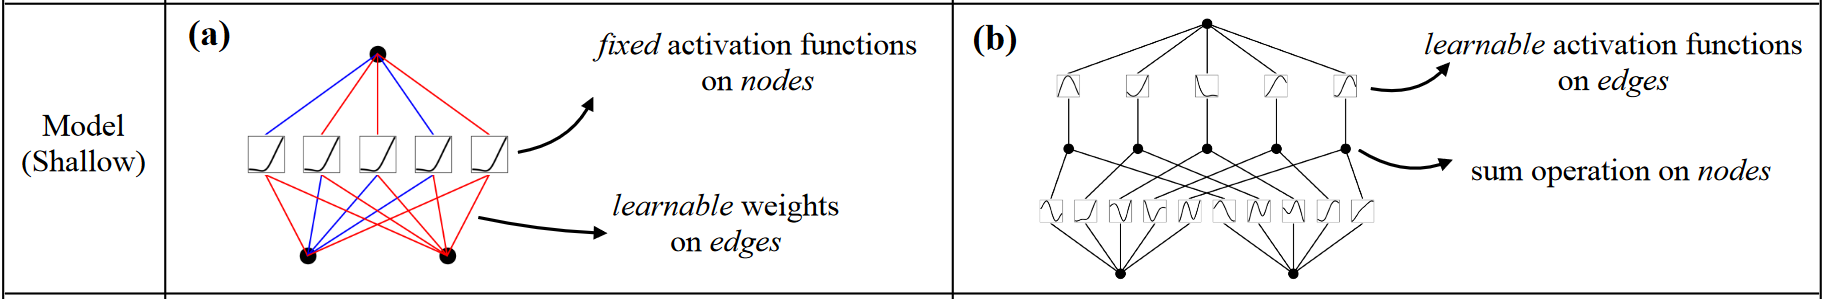
\includegraphics[width=\columnwidth * 2]{figures/kan-network.png}
    \caption{KAN vs MLP Z. Liu et al., “KAN: Kolmogorov-Arnold Networks.” arXiv, May 02, 2024. doi: 10.48550/arXiv.2404.19756.}
    \label{fig:kan}
\end{figure*}


% ** How am i able to do this **
% - transfomers from layers
% - activation functions are used in FFN layer which is implementation of MLP

% ** Motivate choices of activation functions **
% - to compare activation functions I will take existing Hugging face implementation of GPT-NEO and roBERTa and replace the activation function with the one I want to test
% - according to \cite{Mirzadeh2023} I want to test how much worse ReLU is, then compare with relu with learnable parameters PReLU (explain prelu)
% - according to [reference to swish paper] I want to test swish, to get baseline start with SiLU then compare with swish (explain swish)
% - according to [reference to GeGLU paper] I want to test GeGLU, to get baseline start with GELU then compare with GeGLU (explain GeGlU)
% - parametrize GELU with learnable to comapre against GELU (explain how i parametrized gelu)
% - if all that successfull make parametrized GeGLU
% - lastly to compare KAN network against all of the above 

% ** How to kan **
% - implementation exists by the authors of the paper 
% - seems to be running into a bunch of issues and is very slow
% - using efficient kan impelementation isntead
% - have to decide on some paratmees grid: int the number of grid intervals and k: the order of piecewise polynomial, will use 3 and 5 based on the paper 
\section{Approach} % PAST TENSE!!!
\label{sec:approach}
The transformer structure (as introduced in section \ref{sec:background}) allows the default activation functions to be switched out with different activation functions for testing, enabling a direct comparison of their performance while keeping the rest of the architecture the same. To explore the effectiveness of various activation functions, we will modify the existing Hugging face implementations of \textsc{GPTNeo} \cite{huggingfaceNEO} and \textsc{RoBERTa} \cite{huggingfaceRoberta}.

\subsection{Choosing activation functions}
% The activation functions that will be evaluated are the following: ReLU, SiLU, Swish, PReLU, GELU, GEGLU, learnable GELU and learnable GEGLU. Additionaly the KAN network will be compared against all of those options. 
The activation functions evaluated were Rectified Linear Unit (\textsc{ReLU}) \footnote{PyTorch Library, "torch.nn.ReLU," \textit{PyTorch Documentation}, https://pytorch.org/docs/stable/generated/torch.nn.ReLU.html}, Sigmoid Linear Unit (\textsc{SiLU}) \cite{Hendrycks2023}, Gated SiLU with learnable parameters (\textsc{Swish}) \cite{eger_is_2019}, Parametric ReLU (\textsc{PReLU}) \footnote{PyTorch Library, \textit{torch.nn.ReLU}, PyTorch Documentation, \url{https://pytorch.org/docs/stable/generated/torch.nn.ReLU.html}.}, Gaussian Error Linear Unit (\textsc{GELU}) (baseline models), \textsc{Adaptable GELU}. Additionally, the Kolmogorov–Arnold Networks \textsc{KAN network} \cite{Liu2024} will be compared against all of these options.

\subsubsection{GELU}
Currently, the most popular activation function in LLMs is also used as the default activation function in the baseline models \textsc{GPT-NEO} and \textsc{roBERTa}. It is a smooth approximation of \textsc{ReLU}, originally defined as \(\text{GELU}(x) = x \cdot \Phi(x)\), where \(\Phi(x)\)
is the Cumulative Distribution Function for the Gaussian Distribution. For optimization purposes, since calculating \(\Phi(x)\) is computationally expensive, it is instead calculated with the \textsc{tanh} approximation as:

\(\text{GELU}(x) = 0.5x \left(1 + \tanh\left(\sqrt{\frac{2}{\pi}} \left(x + 0.044715x^3\right)\right)\right)\) \cite{Hendrycks2023}. 

This function will serve as the baseline for comparing all other activation functions, with a particular focus on evaluating it against the novel Learnable GELU.

\subsubsection{ReLU and PReLU}
\textsc{ReLU} was considered state-of-the-art at the time of the original transformer paper \cite{Vaswani2017}, but has since been surpassed by other activation functions.

\[
\text{ReLU}(x) = \max(0, x)
\]

\textsc{ReLU} will be used for comparison with \textsc{PReLU} and \textsc{GELU}. The comparison with \textsc{GELU} is motivated by the findings of \textit{I. Mirzadeh et al.} \cite{Mirzadeh2023}, which suggests that the use of ReLU is acceptable as the impact of activation functions diminishes with increasing model size. The objective is to assess the extent to which \textsc{ReLU} underperforms compared to \textsc{GELU} when applied to smaller models.

\textsc{PReLU} is a variant of \textsc{ReLU} that incorporates learnable parameters, allowing the activation function to adaptably learn the optimal slope for negative values.
\[
\text{PReLU}(x) = \max(0, x) + a \min(0, x)
\]

where a is a learnable parameter. This introduces x learnable parameters where x is the FFNs’ intermediate size in the transformer. The objective is to evaluate whether adding a learnable parameter to \textsc{ReLU} can enhance performance or increase the training time.

\subsubsection{SiLU and Swish}
\textsc{SiLU} was evaluated on LLMs in the original \textsc{GELU} paper \cite{Hendrycks2023} but was found to perform worse than the \textsc{GELU} activation function. It is defined as 
\[
\text{SiLu}(x) = x \cdot \sigma(x), \text{ where } \sigma(x) \text{ is the logistic sigmoid.}
\]
It will be used only as a baseline comparison for the \textit{Swish} activation function, which is its adaptable counterpart with learnable parameters, aiding the objective of exploring the impact of adding learnable parameters to activation functions. 

\textit{Swish} is a self-gated activation function that was proposed by \textit{Ramachandran et al.} \cite{Ramachandran2017}. It was implemented as proposed in a paper
\[
    \text{swish}(x) = x \cdot \text{silu}(\alpha \cdot x)
\]
where \(\alpha\) is a learnable parameter. The objective is to evaluate whether the \textsc{Swish} activation function outperforms the non-adaptable \textsc{SiLU} to evaluate the impact of adding learnable parameters to activation functions.

\subsubsection{Adaptable GELU}
The GELU activation function will be parameterized with learnable parameters. The implementation will be based on the PyTorch GELU implementation[cite] with \textsc{tanh} approximation, which, out of the box, does not support learnable parameters. This approach appears to be novel, as no prior research has been found that explores the impact of adding learnable parameters to the \textsc{GELU} activation function. The new \textsc{GELU} activation function adds a learnable parameter as a scaling factor and is defined as follows:

\[
    0.5 \cdot \alpha \cdot \text{x} \cdot \left( 1.0 + \tanh \left( \sqrt{\frac{2.0}{\pi}} \cdot (\text{x} + 0.044715 \cdot \text{x}^3) \right) \right)
\]

where \(\alpha\) is a learnable parameter. 

This activation function adds a total of 2048 learnable parameters. The objective is to evaluate whether the \textsc{Adaptable GELU} activation function outperforms the standard \textsc{GELU} activation function to evaluate the impact of adding learnable parameters to activation functions.

% \subsubsection{GEGLU and Learnable GEGLU}
% The \textit{GEGLU} activation function is a variant of the GELU activation function that incorporates a gating mechanism as proposed by \textit{Shazeer et al.} \cite{Shazeer2020}. It promises to improve the performance of the GELU activation function by adding a gating mechanism. The GEGLU activation function was implemented as used by 2023 BabyLM winner \cite{Samuel2023} \cite{ltg-bert}:
% \begin{lstlisting}[language=Python, caption={Implementation of GeGLU}]
%     class GeGLU(nn.Module):
%      def forward(self, x):
%          x, gate = x.chunk(2, dim=-1)
%          x = x * F.gelu(gate, approximate='tanh')
%          return x
% \end{lstlisting}

% The \textit{Learnable GEGLU} activation function is an enhanced variant of the GEGLU activation function, incorporating a learnable parameter following the same idea as Learnable GEGLU. This implementation extends the standard GEGLU by introducing a learnable scaling factor, making it a novel approach. The new Learnable GEGLU activation function is defined as follows:

% \begin{lstlisting}[language=Python, caption={Implementation of Learnable GeGLU}]
%     def forward(self, input: Tensor) -> Tensor:
%         x, gate = input.chunk(2, dim=-1)
%         x = x * 0.5 * self.beta * gate * (1.0 + torch.tanh(math.sqrt(2.0 / math.pi) * (gate + 0.044715 * torch.pow(gate, 3.0))))
%         return x
% \end{lstlisting}

% The objective is to first evaluate the performance of GeGLU compared to GELU, and then to evaluate the performance of Learnable GeGLU compared to GeGLU. The hypothesis is that Learnable GeGLU will be the best-performing activation function.

% \subsubsection{No Activation Function}
% The \textsc{No Activation Function} will be used as a baseline for comparison with all other activation functions. This baseline will help determine the impact of using an activation function compared to not using one.

\subsubsection{KAN-Network}
The \textsc{KAN network} is a novel activation function that has shown promising results in the literature. The implementation of the \textsc{KAN network} is available by the original authors but has shown to be problematic and slow during our research. Those issues were addressed in efficient-KAN\footnote{\label{footnote:efficient-kan}Blealtan, \textit{Efficient-KAN, GitHub Repository}, 2024. Available at: \url{https://github.com/Blealtan/efficient-kan} (Accessed: 2024-06-03).} implementation, which was the most popular optimization on GitHub of the original KAN paper at the time of this study. This approach requires careful selection of certain parameters, specifically the number of grid intervals and the order of piece-wise polynomials. Based on recommendations from the paper, we will set these parameters to 3 and 5, respectively. The configuration aims to balance performance and computational efficiency, ensuring that the KAN implementation is both effective and practical for the experiments. FFN layers from GPT-NEO and roBERTa both use MLPs in their implementation, which can be directly replaced with efficient-KAN implementation. As the KAN network increases the number of trainable parameters in the FFNs from 2 million to just over 8 million, the intermediate size for models with the KAN network was reduced to 256 to maintain approximately 2 million parameters in the FFNs. Although this reduction in intermediate size limits the expressiveness of the FFNs, the splines in the KAN network might compensate for this bottleneck.
The objective is to evaluate the performance of the KAN network compared to the other activation functions and to determine whether it is a viable alternative for MLPs in LLMs. Additionally, the \textsc{KAN network} offers the unique capability to extract symbolic representations of the learned activation functions from splines. It also provides the ability to retrain or further train specific parts of the network if necessary. Unfortunately, due to time constraints and the current implementation, this aspect will not be explored in this study. For further discussion, see Section \ref{sec:discussion}.
%\section{Methodology, Background, Problem Description}
Choose one that fits your research best:
\subsection{Methodology and/or background}
Typically in general research articles, the second section contains a description of the research methodology, explaining what you, the researcher, is doing to answer the research question(s), and why you have chosen this method.
For purely analytical work this is a description of the data collection or experimental setup on how to test the hypothesis, with a motivation.

In any case this section includes references to necessary background information.
For a survey paper this includes the method of how you arrived at the set of papers included in the survey.

\subsection{Formal Problem Description}
For some types of work in computer science the methodology is standard: analyze the problem (e.g., make assumptions and derive properties), present a new algorithm and its theoretical background, proving its correctness, and evaluate unproven aspects in simulation.
Then an explanation of the methodology is often omitted, and the setup of the evaluation is part of a later section on the evaluation of the ideas.\footnote{This already shows that there is no single outline to be given for all papers.}
In this case, explain relevant (background) concepts, theory and models in this section (with references) and relate them to your research question.
Also this section then typically contains a more precise, formal description of the problem.

Do not forget to give this section another name, for example after the problem you are solving.

%
%\section{Your contribution (replace this section title by something more informative)}
In computer science typically the third section contains an exposition of the main ideas, for example the development of a theory, the analysis of the problem (some proofs), a new algorithm, and potentially some theoretical analysis of the properties of the algorithm.

Do not forget to give this section another name, for example after the method or idea you are presenting.

Some more detailed suggestions for typical types of contributions in computer science are described in the following subsections.


\subsection*{Experimental work}
In this case, this section will mostly contain a description of the methods/algorithms you will be comparing. Although not all methods need to be described in detail (providing appropriate references are available), make sure that you reveal sufficient details to a reader not familiar with these methods to: a) obtain a high-level understanding of the method and differences between them, and b) understand your explanation of the results/conclusions.

\subsection*{Improvement of an idea}
In this case, you would need to explain in detail how the improvement works. If it is based on some observation that can be proven, this is a good place to provide that proof (e.g., of the correctness of your approach). 

\subsection*{Literature survey}
If your contribution is a literature survey, then the organization of these ``middle'' sections very much depends on the way you want to present/organize the literature you are discussing.
First try to cluster papers that are similar in some aspect. Then think of how these clusters are related, from that you can think of a good order to discuss these clusters; this is sometimes called a bottom-up approach to writing a paper.

In addition, you may try to think about the organization of the literature from a top-down perspective: try to ``take a step back'' and think about the field and what important questions/variants are and build a hierarchical categorization of the field.

Make clear what your contribution is here: a new organization of the literature, identification of open problems/challenges, new parallels/generalizations, a table with pros/cons of different methods, etc.\ 


%
% Define the research questions clearly. Discuss the specific configurations you have settled on, and
% elaborate on the data sets you have utilized. Document the evaluation setup and define the metrics.
% ● 4.1 Research Questions
% ● 4.2 Dataset
% ● 4.3 Models
% ● 4.4 Evaluation Setting and Metrics.
% Evaluation Metrics: You should mention the components of the BabyLM evaluation pipeline; but can defer
% explaining each (fine-tune) task in detail to the BLiMP/GLUE/SuperGLUE papers. However, you should
% describe the process each of these components uses to return a score (i.e. how is the final score
% computed?)
% Evaluation Settings: hardware.
% ● 4.5 Configuration and Implementation Details

\section{Experimental setup}
** Research Questions **
- Does choice of activation function matter in smaller language models?
- sub1: How do adaptable activation functions with learnable parameters compare to their static counterparts?
- sub2: Does use of KAN network instead of MLP improve performance of smaller language model?

** Dataset ** 
- tiny stories
- why tiny storeis and not some other dataset 

** Models ** 
- Hugging face GPT-NEO as baseline encoder and RoBERTa as baseline decoder

** Other utils ** 
- %https://github.com/ltgoslo/ltg-bert/blob/main/training/model.py#L14
- https://github.com/Blealtan/efficient-kan
- https://pytorch.org/docs/stable/generated/torch.nn.PReLU.html#torch.nn.PReLU
- http://arxiv.org/abs/1710.05941
- assumptions or constanst use when applyign kan network and activation functions 

** Hardware ** 
- A100

** Evaluation ** 
- BLiMP - %average of ( anaphor_agreement:, argument_structure:, binding:, control_raising, determiner_noun_agreeme, ellipsis:, filler_gap:, irregular_forms:, island_effects:, npi_licensing:, quantifiers:, subject_verb_agreement:)
- SuperGLUE
% Comparisons
% Gelu (baseline) with Adaptive gelu
% ReLU with PReLU (Adaptive reslu)
% SiLU with Swish
% ReLU with GeLu
\section{Results} % PAST TENSE!!!
\label{sec:results}
\textbf{ToDo: Fix the postition of all those tables bellow.}
All results of evaluations on BLiMP and GLUE datasets are shown in Table \ref{table:all-results}.\\
After performing bootstrap resampling for 10 000 samples, we calculated the mean difference and confidence interval to make each of the comparisons mentioned in section \ref{sec:experimental_setup}.\\
Comparison of Baseline (GELU) model with Adaptive GELU model showed that the mean difference is negative for both BLiMP and GLUE benchmarks, showing that the Adaptive GELU model performed slightly better than the Baseline (GELU) model. However the confidence intervals for both benchmarks contain zero, which means that the difference is not statistically significant. The results are shown in Table \ref{tab:comparison}.\\\\
Boostrap comparing static activations ReLU and SiLU with their adaptive counterparts PReLU and Swish showed that the mean difference is positive for both BLiMP and GLUE benchmarks, showing that the static activation functions performed slightly better than the adaptive activation functions. However the confidence intervals for both benchmarks contain zero, which means that the difference is not statistically significant. The results are shown in Table \ref{tab:comparison-static-adaptive}.\\\\
The highest GLUE score was achieved by the BERT-KAN model with 63.65, the highest BLiMP score was achevied by the GPT-KAN model with 63.43. \textbf{ToDo: Further discuss after all statistical tests are done.}\\\\
Across all models, the training times were relatively consistent, with two outliers: KAN network models and ReLU models. The prolonged training time for the ReLU models might be attributed to the busy DelftBlue nodes, whereas the extended time for the KAN models is expected. We will compute the standard deviations for all models once we obtain all the results. Excluding the two outliers, the standard deviation in training times was 3 minutes and 33 seconds.
\textbf{ToDO: Add results of other comparisons. (evaluations still running on DelftBlue)}

\begin{table}[h]
    \centering
    \begin{tabular}{|l|c|c|}
    \hline
     & \textbf{Blimp} & \textbf{Glue} \\ \hline
    \textbf{Mean difference} & -0.135 & -0.878 \\ \hline
    \textbf{Confidence intervals} & $[-1.16, 0.636]$ & $[-2.674, 0.604]$ \\ \hline
    \end{tabular}
    \caption{Mean differences of combined GPT-Neo and RoBERTa scores for Basline (GELU) and Adaptive (GELU) models}
    \label{tab:comparison}
\end{table}

\begin{table}[h]
    \centering
    \begin{tabular}{|l|c|c|}
    \hline
     & \textbf{Blimp} & \textbf{Glue} \\ \hline
    \textbf{Mean difference} & 0.442 & 1.355 \\ \hline
    \textbf{Confidence intervals} & $[-1.85,  2.3]$ & $[-0.35,  3.05]$ \\ \hline
    \end{tabular}
    \caption{Mean differences of combined GPT-Neo and RoBERTa scores for Static and Adaptive activation functions.}
    \label{tab:comparison-static-adaptive}
\end{table}

\begin{table}[!htp]\centering
    \scriptsize
    \begin{tabular}{lrrrrr}\toprule
    \textbf{Model} &\textbf{Seed} &\textbf{Blimp} &\textbf{Glue} &\textbf{Time} \\\cmidrule{1-5}
    BERT Baseline GELU &42 &54.94 &49.22 & \\
    BERT Baseline GELU &2 &59.5 &59.9 &1h 41m 32s \\
    BERT Baseline GELU &3 &59.6 &56.6 &1h 41m 4s \\
    BERT Baseline GELU &4 &59.3 &57 &1h 41m 5s \\
    BERT Baseline GELU &5 &59.1 &57.5 &1h 42m 21s \\
    GPT Baseline GELU &42 &59.05 &58.22 & \\
    GPT Baseline GELU &1 &58 &58.5 &1h 43m 35s \\
    GPT Baseline GELU &2 &56.6 &57.8 &1h 45m 19s \\
    GPT Baseline GELU &3 &56.6 &59.1 &1h 41m 44s \\
    GPT Baseline GELU &4 &59.2 &60.5 &1h 40m 12s \\
    GPT Baseline GELU &5 &57.4 &59.6 &1h 42m 32s \\
    BERT Adaptive GELU &42 &59.4 &57.1 &1h 58m 39s \\
    BERT Adaptive GELU &1 &59.8 &56.2 &1h 45m 56s \\
    BERT Adaptive GELU &2 &59.3 &59.7 &1h 45m 55s \\
    BERT Adaptive GELU &3 &59 &57 &1h 45m 35s \\
    BERT Adaptive GELU &4 &58.2 &57 &1h 45m 56s \\
    BERT Adaptive GELU &5 &59.8 &59.2 &1h 45m 39s \\
    GPT Adaptive GELU &42 &56.8 &60.2 &1h 43m 41s \\
    GPT Adaptive GELU &1 &56.3 &58.8 &1h 41m 26s \\
    GPT Adaptive GELU &2 &57.4 &58.7 &1h 42m 53s \\
    GPT Adaptive GELU &3 &58.7 &59.6 &1h 41m 11s \\
    GPT Adaptive GELU &4 &56 &59.2 &1h 41m 27s \\
    GPT Adaptive GELU &5 &58.3 &59.3 &1h 41m 19s \\
    \toprule \textbf{Other models (not evaluated on multiple seeds yet) } & & & & \\ \midrule
    BERT ReLU &42 &58.5 &57.2 &2h 24m 46s \\
    BERT PReLU &42 &57 &57.6 &1h 47m 27s \\
    GPT ReLU &42 &56.6 &59.9 &2h 17m 4s \\
    GPT PReLU &42 &59.2 &56.1 &1h 42m 28s \\
    BERT SiLU &42 &58.3 &57.5 &1h 45m 4s \\
    BERT Swish &42 &58 &57.8 &1h 43m 8s \\
    GPT SiLU &42 &56.3 &59.9 &1h 39m 35s \\
    GPT Swish &42 &53.7 &57.6 &1h 39m 22s \\
    BERT KAN &42 &56.69 &63.65 &2h 52m 11s \\
    GPT KAN &42 &63.43 &48.8 &3h 23m 35s \\
    \bottomrule
    \end{tabular}
    \caption{All evaluation results}\label{table:all-results}
\end{table}

\begin{table}[h!]
    \centering
    \begin{tabular}{|l|c|}
    \hline
    \textbf{Model Name} & \textbf{Training Time} \\ \hline
    GPT Baseline GELU & 1h 42m 41s $\pm$ 1m 43s \\ \hline
    BERT Baseline GELU & 1h 41m 27s $\pm$ 32s \\ \hline
    BERT Adaptive GELU & 1h 47m 56s $\pm$ 5m 13s \\ \hline
    GPT Adaptive GELU & 1h 41m 59s $\pm$ 1m 02s \\ \hline
    GPT-ReLU & 2h 17m 4s \\ \hline
    BERT-ReLU & 2h 24m 46s \\ \hline
    BERT-Swish & 1h 43m 8s \\ \hline
    GPT-Swish & 1h 39m 22s \\ \hline
    BERT-PReLU & 1h 47m 27s \\ \hline
    GPT-PReLU & 1h 42m 28s \\ \hline
    KAN2-GPT & 3h 23m 35s \\ \hline
    BERT-kan2 & 2h 52m 11s \\ \hline
    GPT-SiLU & 1h 39m 35s \\ \hline
    BERT-SiLU & 1h 45m 4s \\ \hline
    \end{tabular}
    \caption{Mean training times with standard deviations ToDo: add other SDs and mean times when other evaluations complete.}
    \label{tab:training-times}
\end{table}
\newpage
%
%
%
\section{Discussion} % PRESENT TENSE!!!
\label{sec:discussion}
% TODO: Statistical significance analysis of results and discussion of application of findings.
% % bulletpoint list in latex
% \begin{itemize}
%     \item implications
%     \item threats to validity
%     \item future work
% \end{itemize}

\subsection{Implications}
Our results indicate that the choice of activation functions remains irrelevant even at smaller scales. All comparisons in section \ref{sec:results} show statistically insignificant differences, with a few exceptions unrelated to the research questions. This suggests that the activation function choice does not significantly impact the performance of language models with 10 million parameters. These findings add to the findings of Mirzadeh et al. \cite{Mirzadeh2023}, which suggested the impact of activation functions diminishes as the model size increases. Our results imply that this impact is negligible even at smaller scales, given our experimental setup and hyperparameters.

Regarding the second research question, the results show that parameterizing activation functions does not affect performance, explaining the lack of literature on adaptable activation functions in LMs. More interestingly, our results of comparison between ReLU and GELU challenge the conclusions of Hendrycks et al. \cite{Hendrycks2023}, who claimed GELU's superiority over ReLU. Our results align with Mirzadeh et al. \cite{Mirzadeh2023}, who advocate for ReLU's return. While our research does not necessitate a return to ReLU, it also does not provide strong arguments for preferring GELU over ReLU or PReLU.

A likely reason for this outcome is that the models were trained for only one epoch, preventing them from converging, and making the results rather inconclusive. See further discussion in Section \ref{sec:external} and Section \ref{sec:internal}.

Furthermore, the training durations of models using various activation functions showed minimal differences, indicating that the choice of activation function does not significantly impact training efficiency.

The comparison of results further supports the findings of Dror et al. \cite{dror2018hitchhikers}, which emphasize the importance of statistical significance analysis in evaluating architectural decisions in language models. Some of our findings indicated better performance with certain activations, but subsequent analysis revealed these improvements to be statistically insignificant.

GPT models with KAN networks perform worse than those with traditional MLPs, as indicated by their lowest mean scores on GLUE and most BLiMP benchmarks. While this does not necessarily imply that KAN networks should be avoided, it suggests that the setup used in this research does not lead to improvement. Further research is needed to explore the potential of KAN networks in language models. See Section \ref{sec:future}

\subsection{Threats to validity}
Internal validity examines the certainty that the observed results are due to independent variables and not other factors. External validity concerns the extent to which the findings of the study can be generalized to contexts outside the study. Construct validity refers to the extent to which the measurement tools are appropriate for the study. 

% Limited compute
% only one epoch
% only two different types of models
% we did multiple seeds
\subsubsection{Internal validity}
\label{sec:internal}
To ensure that our results were not due to chance, we trained models using six different random seeds. While this sample size is relatively small, it was a necessary compromise given our resource constraints. To address this limitation, we employed bootstrapping with 10,000 samples to calculate confidence intervals and mean differences between models. Additionally, to verify that our findings were not model-specific, we utilized two distinct types of models: an encoder (roBERTa) and a decoder (GPT-Neo).

Nevertheless, it is important to note that all models were trained on the same dataset, which may have introduced some bias. The training times could have been affected by busy Delft Blue nodes, but across models trained on multiple seeds, the training times were relatively consistent, with a standard deviation of only 9 minutes and 52 seconds across all models, including those with KAN-Networks.

Another potential threat to validity is that the implementation of adaptable activation functions added 2,048 learnable parameters to each model, which could have influenced the results. However, given that 2,048 parameters constitute a relatively small proportion in models with 9 million parameters, and the results were not statistically significant, this impact is likely minimal.

% Tiny stories might not be representative 
% Would be trained on more epochs so models would further converge 
% Kan is new, implementation was not perfect, training was unstable
\subsubsection{External validity}
\label{sec:external}
All the models were trained for only one epoch due to computational constraints, resulting in none of the models fully converging. This may have impacted the performance of the models and the significance of the results, as differences might be more pronounced or minimized with additional epochs. In a real-world scenario, models would typically be trained for more epochs. Additionally, the models utilized in this study are not the latest state-of-the-art, which may affect the generalizability of the results. Furthermore, the TinyStories dataset used for pre-training, which comprises only short fictional stories, may not be representative of the datasets typically used for production-level language models.

The implementation of the KAN-Network\footnotemark[3] used in this study makes certain assumptions to optimize the originally proposed KAN implementation. One key change is the removal of the learnable scale from each activation function to improve efficiency. Additionally, the interpretability of KANs, a notable feature in the original design, is compromised in this implementation. This is because the critical L1 regularization, which was originally applied to input samples, has been moved to the weights. While this adjustment aligns better with common neural network practices and is compatible with the rest of the transformer architecture, it reduces the interpretability highlighted in the original paper and may also affect performance.

\subsubsection{Construct validity}
The evaluation pipeline used in this study, BabyLM, primarily focuses on grammatical tasks, which may not fully capture the comprehensive capabilities of language models. However, considering the scope of this research, the tasks evaluated by the BabyLM evaluation pipeline are suitable. Since BabyLM is specifically designed for the evaluation of smaller language models, it aligns well with our study's focus. Thus, it is an appropriate tool for assessing the impact of activation functions on these models.

\subsection{Future work}
\label{sec:future}
I hope this research will inspire further studies to give activation functions less attention. Before publishing new activation functions, researchers should conduct multiple runs and perform statistical significance tests to ensure the robustness of their findings. \\ 
The KAN architecture is a relatively new concept, and the implementation used in this study may not have been optimal. Although we utilized more efficient and optimized implementation as suggested by the original paper \cite{Liu2024}, the training process was less stable compared to baseline models (see Figure \ref{fig:grad-norm}), and the models did not converge as expected. This instability may have impacted the performance of the \textsc{KAN models}, suggesting that future research should investigate this issue further. Despite its potential, this promising direction concerning activation functions and its interpretability benefits were not fully explored in this study due to time constraints.

\begin{figure}[ht]
    \centering
    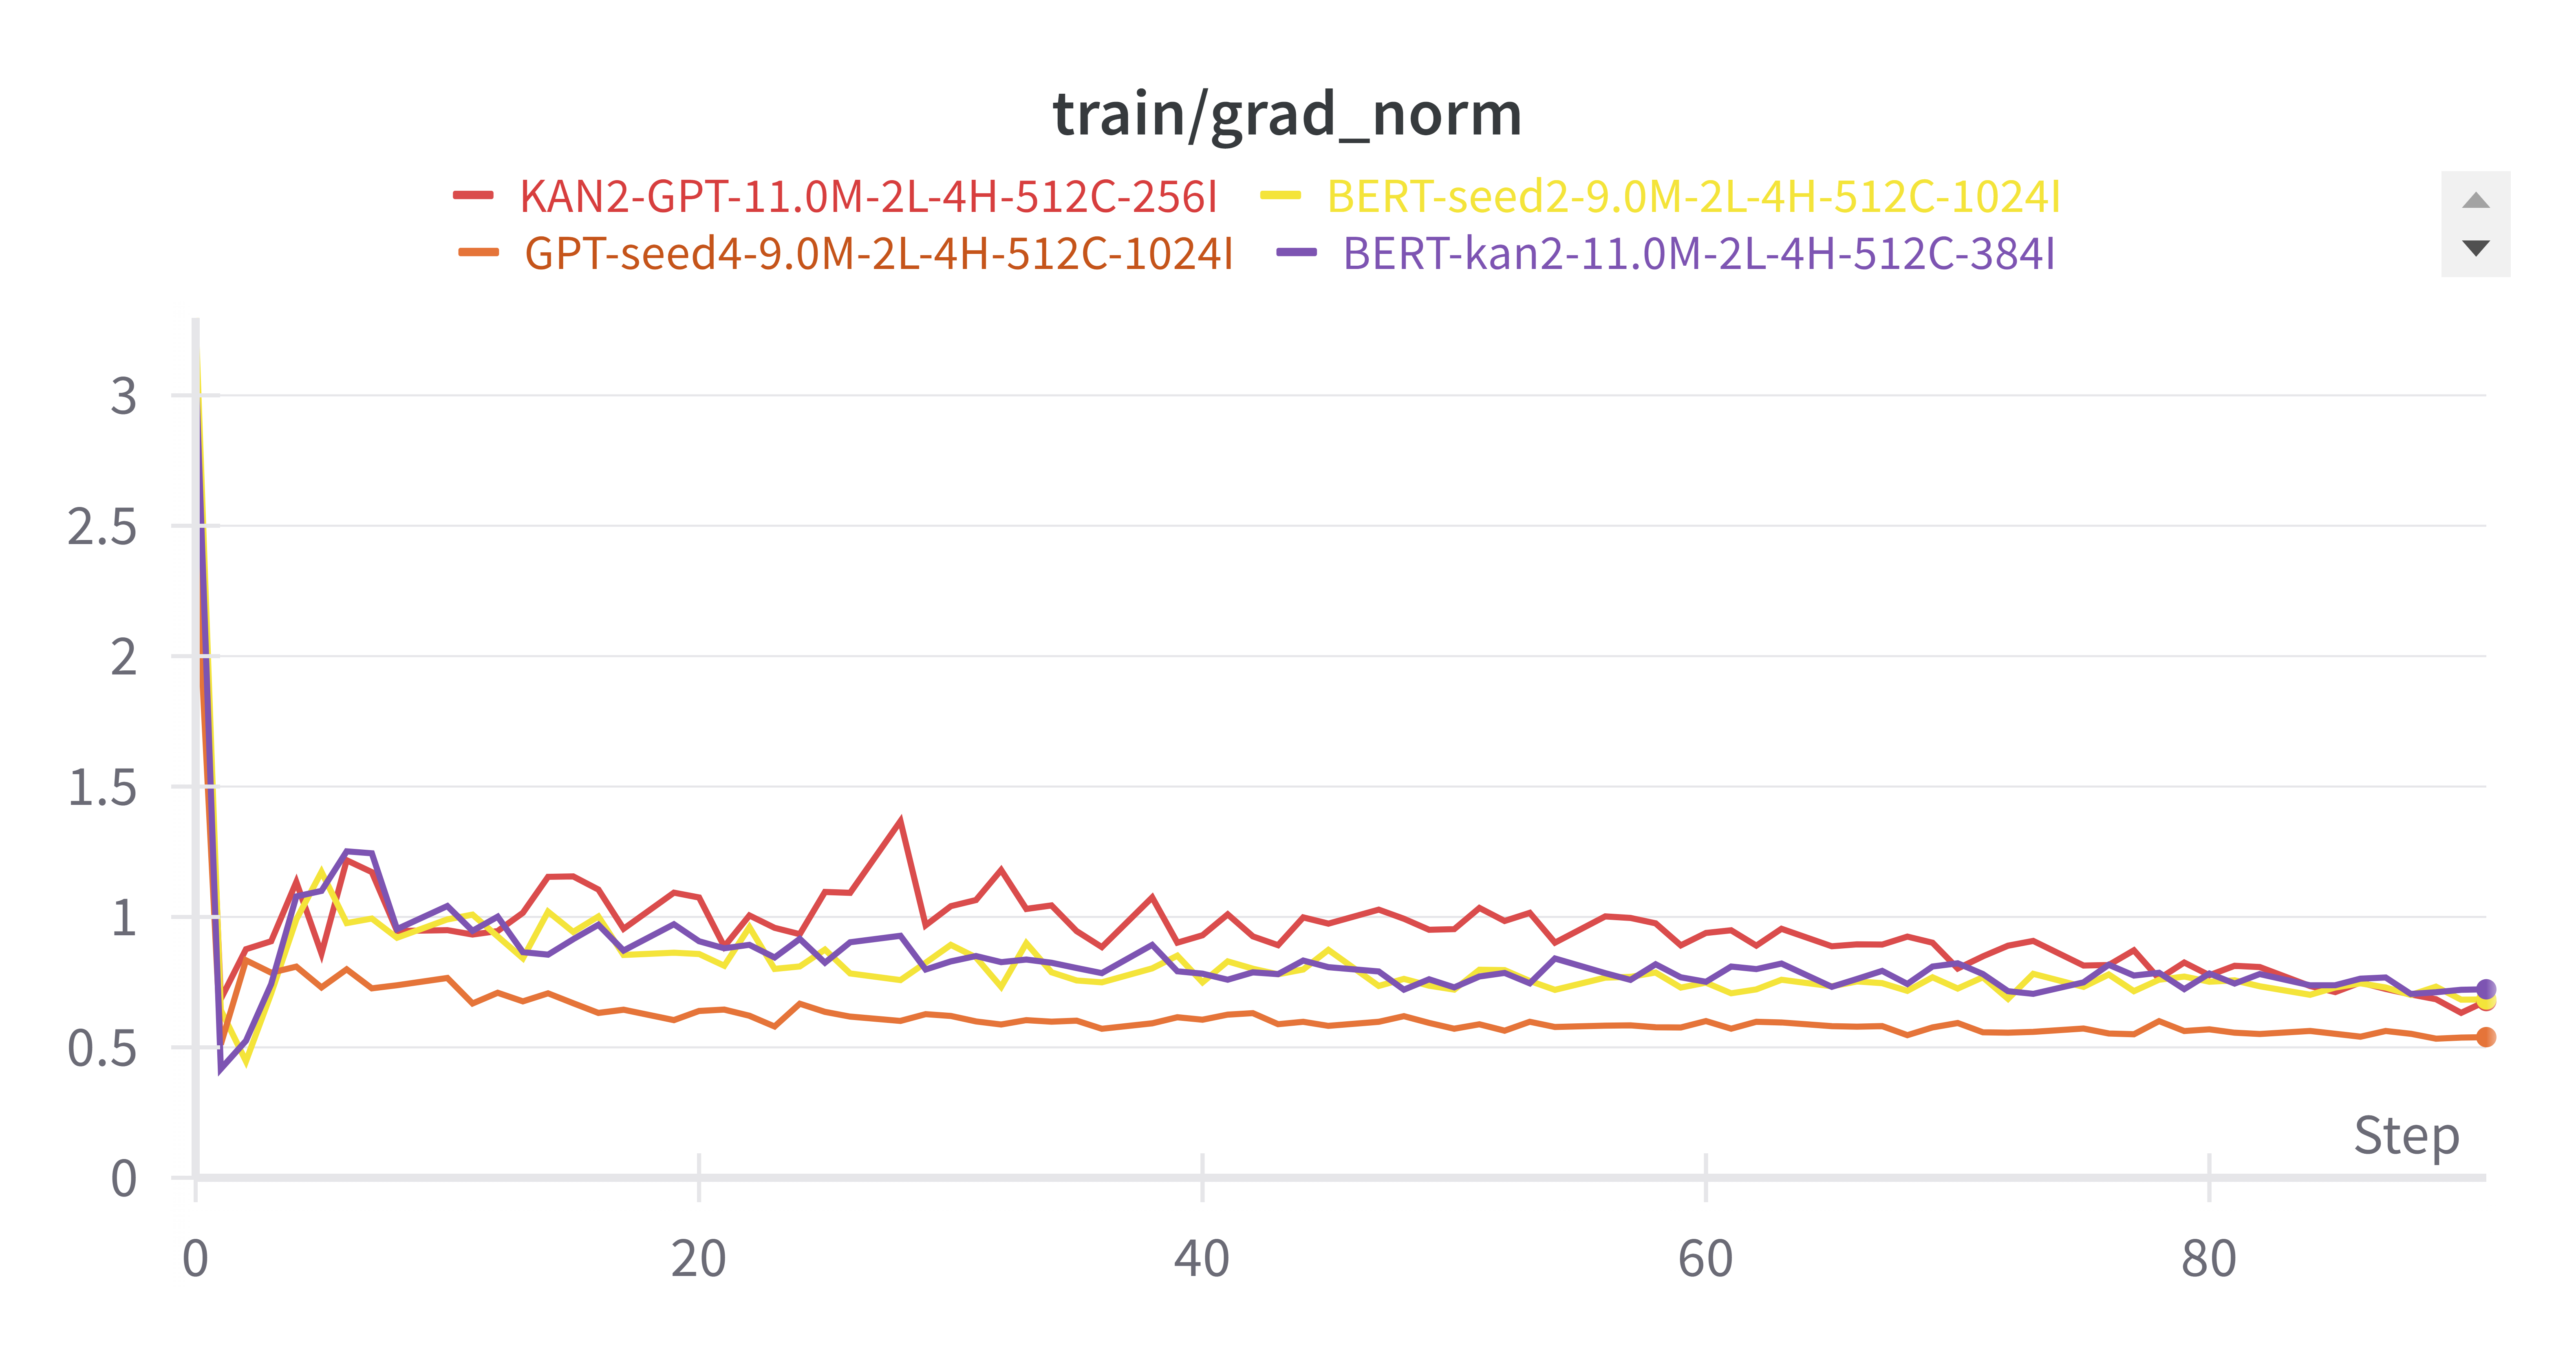
\includegraphics[width=\columnwidth]{figures/train-grad-norm.png}
    \caption{Gradient normalization during training of KAN models. The KAN models show higher variance in gradient norms compared to the baseline models. \textbf{ToDo: Fix readability}}
    \label{fig:grad-norm}
\end{figure}

%
\section{Conclusions and Future Work} % PRESENT TENSE!!!
\textbf{TODO:}
% bullet points of conclusions
\begin{itemize}
    \item brielfy repeat the RQs
    \item Discuss the the implications of results
    \item Suggest future research directions
\end{itemize}
%
%\newpage
\section{Appendix}
\label{Appendix}
%If the table is too wide, replace \begin{table}[!htp]...\end{table} with
%\begin{adjustwidth}{-2.5 cm}{-2.5 cm}\centering\begin{threeparttable}[!htb]...\end{threeparttable}\end{adjustwidth}

\begin{table}[!htp]\centering
    \caption{Bootstraped means of GLUE and BLiMP with 95\% confidence intervals}
    \label{tab:bootstraped-means }
    \scriptsize
    \begin{tabular}{lrrrrr}\toprule
    Model &Glue Mean &95\% CI Glue &Blimp Mean &95\% CI Blimp \\\cmidrule{1-5}
    BERT Baseline (GELU) &57.44 &[56.52, 58.73] &58.48 &[56.68, 59.5] \\
    BERT Learnable GELU &57.69 &[56.75, 58.73] &59.25 &[58.78, 59.65] \\
    GPT Baseline (GELU) &58.95 &[58.27, 59.7] &57.82 &[56.97, 58.68] \\
    GPT Learnable GELU &59.30 &[58.92, 59.73] &57.24 &[56.47, 58.03] \\
    BERT ReLU &57.91 &[56.98, 58.87] &58.40 &[57.37, 59.23] \\
    BERT PReLU &58.58 &[57.67, 59.28] &58.37 &[57.70, 59.05] \\
    GPT ReLU &59.41 &[59.0, 59.82] &56.91 &[55.93, 57.8] \\
    GPT PReLU &58.83 &[57.6, 59.82] &57.60 &[56.34, 58.83] \\
    BERT SiLU &57.54 &[57.15, 58.1] &59.16 &[58.75, 59.53] \\
    BERT Swish &57.89 &[57.28, 58,48] &58.26 &[57.71, 58.75] \\
    GPT SiLU &59.05 &[58.4, 59.63] &57.25 &[56.43, 58.2] \\
    GPT Swish &58.36 &[57.95, 58,78] &55.64 &[54.68, 56.64] \\
    GPT KAN &55.15 &[52.54, 56.73] &55.38 &[53.68, 56.47] \\
    \bottomrule
    \end{tabular}
\end{table}
    
    \begin{table}[!htp]\centering
        \caption{Average pre-train times and standard devitations for all the models. \textit{Note:} \textbf{*} \textit{indicates models that were trained on V100s instead of A100s due to time constraints and DelftBlue cluster availability.}}
        \label{tab:average-times}
        \scriptsize
        \begin{tabular}{lrr}\toprule
        Model &Avg. Train. Time \\ \cmidrule{1-2}
        BERT Baseline (GELU) &1h 41m 27s ± 32s \\
        BERT Learnable GELU &1h 47m 56s ± 313s \\
        GPT Baseline (GELU) &1h 42m 41s ± 103s \\
        GPT Learnable GELU &1h 41m 59s ± 102s \\
        *BERT ReLU &2h 25m 23s ± 147s \\
        BERT PReLU &1h 46m 11s ± 46s \\
        *GPT ReLU &2h 20m 27s ± 203s \\
        GPT PReLU &1h 41m 23s ± 40s \\
        BERT SiLU &1h 43m 50s ± 268s \\
        *BERT Swish &2h 20m 4s ± 1086s \\
        GPT SiLU &1h 39m 7s ± 270s \\
        *GPT Swish &2h 31m 4s ± 1032s \\
        *GPT KAN &3h 58m 11s ± 2663s \\
        \bottomrule
        \end{tabular}
        \end{table}


\begin{table}[!htp]\centering
    \caption{Pre-Train times, BLiMP and GLUE scores for all the modes. \textit{Note:} \textbf{*} \textit{indicates models that were trained on V100s instead of A100s due to time constraints and DelftBlue cluster availability.}}
    \label{tab:all-results}
    \scriptsize
    \begin{tabular}{lrrrrr}\toprule
    \textbf{Model} &\textbf{Seed} &\textbf{Blimp} &\textbf{Glue} &\textbf{Time} \\\cmidrule{1-5}
    BERT Baseline (GELU) &42 &54.94 &49.22 &1h 41m 16s \\
    BERT Baseline (GELU) &2 &59.5 &59.9 &1h 41m 32s \\
    BERT Baseline (GELU) &3 &59.6 &56.6 &1h 41m 4s \\
    BERT Baseline (GELU) &4 &59.3 &57 &1h 41m 5s \\
    BERT Baseline (GELU) &5 &59.1 &57.5 &1h 42m 21s \\
    GPT Baseline (GELU) &42 &59.05 &58.22 &1h 42m 44s \\
    GPT Baseline (GELU) &1 &58 &58.5 &1h 43m 35s \\
    GPT Baseline (GELU) &2 &56.6 &57.8 &1h 45m 19s \\
    GPT Baseline (GELU) &3 &56.6 &59.1 &1h 41m 44s \\
    GPT Baseline (GELU) &4 &59.2 &60.5 &1h 40m 12s \\
    GPT Baseline (GELU) &5 &57.4 &59.6 &1h 42m 32s \\
    BERT Learnable GELU &42 &59.4 &57.1 &1h 58m 39s \\
    BERT Learnable GELU &1 &59.8 &56.2 &1h 45m 56s \\
    BERT Learnable GELU &2 &59.3 &59.7 &1h 45m 55s \\
    BERT Learnable GELU &3 &59 &57 &1h 45m 35s \\
    BERT Learnable GELU &4 &58.2 &57 &1h 45m 56s \\
    BERT Learnable GELU &5 &59.8 &59.2 &1h 45m 39s \\
    GPT Learnable GELU &42 &56.8 &60.2 &1h 43m 41s \\
    GPT Learnable GELU &1 &56.3 &58.8 &1h 41m 26s \\
    GPT Learnable GELU &2 &57.4 &58.7 &1h 42m 53s \\
    GPT Learnable GELU &3 &58.7 &59.6 &1h 41m 11s \\
    GPT Learnable GELU &4 &56 &59.2 &1h 41m 27s \\
    GPT Learnable GELU &5 &58.3 &59.3 &1h 41m 19s \\
    *BERT ReLU &42 &58.5 &57.2 &2h 24m 46s \\
    *BERT ReLU &1 &58 &58.7 &2h 22m 40s \\
    *BERT ReLU &2 &56.1 &59.6 &2h 25m 13s \\
    *BERT ReLU &3 &59.2 &56.3 &2h 25m 51s \\
    *BERT ReLU &4 &58.7 &58.8 &2h 29m 52s \\
    *BERT ReLU &5 &59.9 &56.8 &2h 23m 59s \\
    *GPT ReLU &42 &56.6 &59.9 &2h 17m 4s \\
    *GPT ReLU &1 &58.5 &58.7 &2h 16m 42s \\
    *GPT ReLU &2 &56.1 &59.6 &2h 21m 34s \\
    *GPT ReLU &3 &57.4 &59.3 &2h 20m 47s \\
    *GPT ReLU &4 &55 &58.9 &2h 25m 58s \\
    *GPT ReLU &5 &57.9 &60.1 &2h 20m 39s \\
    BERT SiLU &42 &58.3 &57.5 &1h 45m 4s \\
    BERT SiLU &1 &58.9 &58.9 &1h 41m 41s \\
    BERT SiLU &2 &59.8 &57.4 &1h 52m 26s \\
    BERT SiLU &3 &59.6 &57.1 &1h 41m 40s \\
    BERT SiLU &4 &59 &57.3 &1h 40m 43s \\
    BERT SiLU &5 &59.4 &57 &1h 41m 26s \\
    GPT SiLU &42 &56.3 &59.9 &1h 39m 35s \\
    GPT SiLU &1 &59.3 &57.7 &1h 37m 5s \\
    GPT SiLU &2 &55.9 &58.5 &1h 48m \\
    GPT SiLU &3 &57.9 &59.7 &1h 36m 55s \\
    GPT SiLU &4 &57.2 &58.9 &1h 37m \\
    GPT SiLU &5 &56.9 &59.6 &1h 36m 7s \\
    BERT Swish &42 &58 &57.8 &1h 43m 8s \\
    *BERT Swish &1 &57.7 &57.3 &2h 26m 13s \\
    *BERT Swish &2 &57.2 &58.9 &2h 27m 10s \\
    *BERT Swish &3 &58.9 &56.8 &2h 27m 48s \\
    *BERT Swish &4 &59 &58.8 &2h 28m 27s \\
    *BERT Swish &5 &58.8 &57.7 &2h 27m 39s \\
    GPT Swish &42 &53.7 &57.6 &1h 39m 22s \\
    *GPT Swish &1 &55 &58.6 &2h 19m 34s \\
    *GPT Swish &2 &56 &59.2 &2h 20m 51s \\
    *GPT Swish &3 &56.4 &57.9 &2h 21m 43s \\
    *GPT Swish &4 &57.2 &57.8 &2h 21m 30s \\
    *GPT Swish &5 &55.6 &59 &2h 23m 24s \\
    BERT PReLU &42 &57 &57.6 &1h 47m 27s \\
    BERT PReLU &1 &59.8 &59.6 &1h 45m 25s \\
    BERT PReLU &2 &58.2 &58.1 &1h 45m 30s \\
    BERT PReLU &3 &58.7 &56.9 &1h 46m 37s \\
    BERT PReLU &4 &58 &59.5 &1h 45m 54s \\
    BERT PReLU &5 &58.5 &59.8 &1h 46m 14s \\
    GPT PReLU &42 &59.2 &56.1 &1h 42m 28s \\
    GPT PReLU &1 &56.2 &59.1 &1h 41m 7s \\
    GPT PReLU &2 &55.5 &60.5 &1h 40m 40s \\
    GPT PReLU &3 &56.6 &59.5 &1h 41m 50s \\
    GPT PReLU &4 &59.6 &58.2 &1h 40m 48s \\
    GPT PReLU &5 &58.5 &59.6 &1h 41m 24s \\
    GPT KAN &42 &63.43 &48.8 &3h 23m 35s \\
    *GPT KAN &1 &52.7 &56.5 &3h 22m 36s \\
    *GPT KAN &2 &53.8 &56.6 &4h 54m 37s \\
    GPT KAN &3 &54.9 &57 &4h 52m 29s \\
    GPT KAN &4 &54.2 &55.4 &3h 23m 10s \\
    GPT KAN &5 &53.2 &56.7 &3h 52m 41s \\
    \bottomrule
    \end{tabular}
    \end{table}

\end{document}
\section{Reponsible research} % PRESENT TENSE!!!
\label{sec:responsible_research}
To prevent test set contamination, we pre-trained our models on datasets that were separate from those used for evaluation. This addresses an issue highlighted in recent works, where pre-training on test sets can artificially inflate performance metrics and call into question the validity of the results \cite{schaeffer2023pretraining}. Ensuring distinct separation between training and evaluation datasets maintains the integrity of our findings and contributes to the reliability of our research.
\\
In conducting this research, we ensured transparency and reproducibility by sharing the experimental setup under section \ref{sec:experimental_setup}. The datasets and models used are publicly available and can be found in the references. Furthermore, all the implemented code is available on GitHub? We adhered to scientific integrity by fabrication, and plagiarism, ensuring that everything reported accurately with proper citations.
\\
Guided by the Netherlands Code of Conduct for Research Integrity, we incorporated principles of honesty, transparency, and responsibility, ensuring our research practices align with the highest standards. We followed the educational and normative framework from chapters 2 and 3 of the Code, emphasizing good research practices that promote a responsible research environment \cite{knaw2018integrity}. 

\newpage
\bibliographystyle{plain}
\bibliography{references}

%A rule of thumb for dealing with the literature is the following: scan about 10--20 contributions: read title, abstract, part of introduction and conclusions; categorize contribution; some of these are studied in more depth: completely read about 5 conference papers or equivalent (summarize contribution in own words); of which studied in-depth about 2 conference papers (the student is able to explain in detail and criticize contributions). This may result in 5--20 references, possibly even more if the project is a literature study.


\end{document}

